\documentclass[../Main.tex]{subfiles}

\begin{document}
\chapter{Mathematical Proofs}

\section{Set Theory}
\textit{\textbf{Set}: A collection of objects considered as a single object.}\\

\begin{itemize}
    \item[$\blacktriangleright$] \textbf{Open Interval $(\, )$}: $(a, b)$ represents all $\Re$ $x$ such that $a < x < b$.
    \item[$\blacktriangleright$] \textbf{Closed Interval $[\, ]$}: $[a, b]$ represents all $\Re$ $x$ such that $a \leq x \leq b$.
    \item[$\blacktriangleright$] \textbf{Half-Open/Half-Closed Intervals}: $[a, b)$ means $a \leq x < b$, and $(a, b]$ means $a < x \leq b$.
\end{itemize}

\textbf{Disjoint:} $A \cap B = \emptyset$\\

\textbf{Difference:} $A-B$ or $A/B$ $= \{x: x\in A$ and $x \notin B \}$\\

\exm{Set operations}{
\quad Let $A = \{x \in \mathbb{R} : |x| \leq 3\}$, $B = \{x \in \mathbb{R} : |x| > 2\}$ and $C = \{x \in \mathbb{R} : |x - 1| \leq 4\}$.
\begin{enumerate}
    \item Express $A$, $B$ and $C$ using interval notation.
    \item Determine $A \cap B$, $A - B$, $B \cap C$, $B \cup C$, $B - C$ and $C - B$.
\end{enumerate}
\textbf{Solution}
\begin{enumerate}
    \item $A = [-3, 3]$, $B = (-\infty, -2) \cup (2, \infty)$ and $C = [-3, 5]$ \textit{(For C, $-4\leq x-1 \leq 4$)}.
    \item $A \cap B = [-3, -2) \cup (2, 3]$, $A - B = [-2, 2]$, $B \cap C = [-3, -2) \cup (2, 5]$, $B \cup C = (-\infty, \infty)$, $B - C = (-\infty, -3) \cup (5, \infty)$ and $C - B = [-2, 2]$.
\end{enumerate}}

\section*{Complement:} All elements that are \textit{not in} the given set but are \textit{within} a defined \textbf{universal set}.\\

Consider universal set $U$. For a set $A$, its \textbf{complement} is: 
$\overline{A} = U - A = \{x : x \in U \text{ and } x \notin A\}$.

If $U = \mathbb{Z}$, then $\overline{\mathbb{N}} = \{0, -1, -2, \dots\}$; while if $U = \mathbb{R}$, then $\overline{\mathbb{Q}} = \mathbb{I}$.

\subsection*{Key Properties of Complements}

Let $U$ be the universal set and $A$ and $B$ be subsets of $U$.

\begin{itemize}
    \item \textbf{Union with Original Set:} A set and its complement, when united, form the universal set:
    \[A \cup \overline{A} = U\]
    \item \textbf{Intersection with Original Set:} A set and its complement are always disjoint (they have no elements in common):
    \[A \cap \overline{A} = \emptyset\]
    \item \textbf{Double Complement:} The complement of the complement of a set is the original set itself:
    \[\overline{(\overline{A})} = A\]
    \item \textbf{Complement of Universal Set:} The complement of the universal set is the empty set:
    \[\overline{U} = \emptyset\]
    \item \textbf{Complement of Empty Set:} The complement of the empty set is the universal set:
    \[\overline{\emptyset} = U\]
    \item \textbf{De Morgan's Laws:} These important laws relate complements to unions and intersections:
    \begin{itemize}
        \item The complement of a union is the intersection of the complements:
        \[\overline{(A \cup B)} = \overline{A} \cap \overline{B}\]
        \item The complement of an intersection is the union of the complements:
        \[\overline{(A \cap B)} = \overline{A} \cup \overline{B}\]
    \end{itemize}
\end{itemize}
%%%%%%%%%%%%%%#############################################

\subsection{Indexed Collections of Sets}
\defn{Union $A \cup B \cup C$}{
\begin{center}
    $A \cup B \cup C = \{x: x\in A_i$ or $ x \in B$, or $x \in C\}$
\end{center}
}

\defn{Union of sets (set of sets)}{
To consider the union of several sets: The union of $n \geq 2$ sets $A_1, A_2, \dots, A_n$ is denoted by $A_1 \cup A_2 \cup \dots \cup A_n$ or $\bigcup_{i=1}^{n} A_i$, 
\[ \bigcup_{i=1}^{n} A_i = \{x : x \in A_i \text{ for some } i, 1 \leq i \leq n\}. \]

Thus, for element $a$ to belong to $\bigcup_{i=1}^{n} A_i$, $a$ must belong to at least one of the sets $A_1, A_2, \dots, A_n$.
}

\exm{Union of sets}{
\quad Let $B_1 = \{1, 2\}$, $B_2 = \{2, 3\}$, \dots, $B_{10} = \{10, 11\}$; that is, $B_i = \{i, i+1\}$ for $i = 1, 2, \dots, 10$. Determine each of the following:
\begin{enumerate}
    \item[(a)] $\bigcup_{i=1}^{5} B_i$.
    \item[(b)] $\bigcup_{i=1}^{10} B_i$.
    \item[(c)] $\bigcup_{i=3}^{7} B_i$.
    \item[(d)] $\bigcup_{i=j}^{k} B_i$, where $1 \leq j \leq k \leq 10$.
\end{enumerate}

\textbf{Solution}
\begin{enumerate}
    \item[(a)] $\bigcup_{i=1}^{5} B_i = \{1, 2, \dots, 6\}$.
    \item[(b)] $\bigcup_{i=1}^{10} B_i = \{1, 2, \dots, 11\}$.
    \item[(c)] $\bigcup_{i=3}^{7} B_i = \{3, 4, \dots, 8\}$.
    \item[(d)] $\bigcup_{i=j}^{k} B_i = \{j, j+1, \dots, k+1\}$. \hfill $\blackdiamond$
\end{enumerate}
}

\subsection{Partitions of Sets}

\textbf{Recall} $2$ sets are disjoint if their intersection is the empty set. A collection $S$ of subsets of a set $A$ is \textbf{pairwise disjoint} if every $2$ distinct subsets that belong to $S$ are disjoint.
($element_1 \cap element_2 \cap element_n = \emptyset$).

\textbf{Partition of $A$:} Collection $S$ of nonempty subsets of $A$ such that $\forall x_i \in A$ belongs exactly $1$ subset in $S$.

\begin{enumerate}
    \item $X \neq \emptyset$ $\forall set X \in S$ 
    \item for every $2$ sets $X,Y \in S$, either $X=Y$ or $X \cap Y = \emptyset$
    \item $\bigcup_{X \in S}X=A$
\end{enumerate}

\exm{Partition}{
Consider collection of subsets of set $A = \{1,2,3,4,5,6\}$:
\begin{align*}
S_1 &= \{\{1, 3, 6\}, \{2, 4\}, \{5\}\}; \\
S_2 &= \{\{1, 2, 3\}, \{4\}, \emptyset, \{5, 6\}\}; \\
S_3 &= \{\{1, 2\}, \{3, 4, 5\}, \{5, 6\}\}; \\
S_4 &= \{\{1, 4\}, \{3, 5\}, \{2\}\}.
\end{align*}
\textit{Determine which of these sets are partitions of $A$.}\\

\begin{solution}
The set $S_1$ is a partition of $A$. The set $S_2$ is not a partition of $A$ since $\emptyset$ is one of the elements of $S_2$. Set $S_3$ is not a partition of $A$ since the element 5 belongs to two distinct subsets in $S_3$ ($\{3, 4, 5\}$, $\{5, 6\}$). $S_4$ is not a partition of $A$ because element 6 belongs to no subset in $S_4$. \rule{0.5em}{0.5em}
\end{solution}

A partition of a nonempty set $A$ is a division of $A$ into nonempty subsets.\\

\textbf{Partition $S_1$ of set $A$:}

\begin{center}
    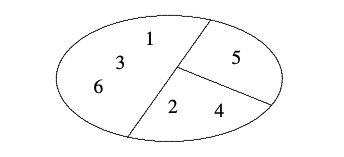
\includegraphics[scale=0.6]{files/partition.png}
\end{center}

The set $\mathbb{Z}$ of integers can be partitioned into the set of even integers and the set of odd integers. The set $\mathbb{R}$ of real numbers can be partitioned into the set $\mathbb{R}^+$ of positive real numbers, the set of negative real numbers and the set $\{0\}$ consisting of the number $0$. $\mathbb{R}$ can also be partitioned into the set $\mathbb{Q}$ of rational numbers and the set $\mathbb{I}$ of irrational numbers.
}

\subsection{Cartesian Products of Sets}

The \textbf{Cartesian product} $A *B$ of $2$ $sets$ $A$ and $B$ is the set consisting of all \textbf{ordered pairs} whose first coordinate belongs to $A$ and whose second belongs to $B$:\\

$A*B = \{(a,b): a \in A$ and $b \in B\}$

\exm{Cartesian}{
If $A = \{x, y\}$ and $B = \{1, 2, 3\}$, then
\begin{align*}
A \times B &= \{(x, 1), (x, 2), (x, 3), (y, 1), (y, 2), (y, 3)\}, \\
\intertext{while}
B \times A &= \{(1, x), (1, y), (2, x), (2, y), (3, x), (3, y)\}.
\end{align*}
Since, for example, $(x, 1) \in A \times B$ and $(x, 1) \notin B \times A$, these two sets do not contain the same elements; so $A \times B \ne B \times A$. Also,
\begin{align*}
A \times A &= \{(x, x), (x, y), (y, x), (y, y)\} \\
\intertext{and}
B \times B &= \{(1, 1), (1, 2), (1, 3), (2, 1), (2, 2), (2, 3), (3, 1), (3, 2), (3, 3)\}. \quad \blacksquare
\end{align*}

Note if $A = \emptyset$ or $B = \emptyset$, then $A \times B = \emptyset$.
The Cartesian product $\mathbb{R} \times \mathbb{R}$ is the set of all points in the Euclidean plane. \\

Consider: The graph of the straight line $y = 2x + 3$ is the set
\[
\{(x,y) \in \mathbb{R} \times \mathbb{R} : y = 2x + 3\}.
\]
For the sets $A = \{x, y\}$ and $B = \{1, 2, 3\}$, $|A|=2$ and $|B|=3$; while $|A \times B| = 6$. Indeed, for all finite sets $A$ and $B$,
\[
|A \times B| = |A| \cdot |B|.
\]
}
% \textit{Further explanation for $(d)$}: Find \textbf{intersection} of $B_i$ from $i=j$ to $i=k$. Thus goal is to look for elements present in $B_j,B_{j+1},…,B_k$.\\

% \textbf{Consider:} \\

% \textbf{Case 1:} $k=j+1$ $\rightarrow$ Find all uniquebetween 2 consecutive sets: $B_j, B_{j+1}$
% \begin{center}
%     $B_j = \{j,j+1\}$\\
%     $B_{j+1} = \{j +1,j+2\}$\\
%     Therefore, if $k=j+1$, $B_j \cap B_{j+1} = \{j+1\}$  
% \end{center}




\end{document}

